\documentclass[tikz]{standalone}
\usepackage{tikz}

\begin{document}
	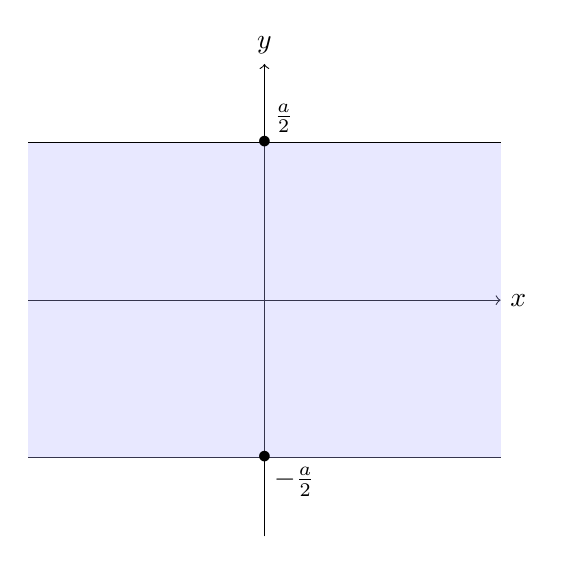
\begin{tikzpicture}
		\draw[->] (-3, 0) -- (3, 0) node[right] {$x$};
		\draw[->] (0, -3) -- (0, 3) node[above] {$y$};
		\draw (-3, 2) -- (3, 2);
		\draw (-3, -2) -- (3, -2);
		\fill[opacity=0.3,blue!30] (-3,-2) rectangle (3,2);
		\draw(0,2) node {$\bullet$};
		\draw(0,2) node[above right]{$\frac{a}{2}$};
		\draw(0,-2) node {$\bullet$};
		\draw(0,-2) node[below right]{$-\frac{a}{2}$};
	\end{tikzpicture}
\end{document}